\documentclass{article}

%% begin preamble

\usepackage[utf8]{inputenc}  % input encoding utf-8
\usepackage[T1]{fontenc}  % font encoding - T1

\usepackage{fullpage}  % for narrower margins
\usepackage{hyperref} % for urls 
\usepackage{booktabs} % For \toprule, \midrule and \bottomrule
\usepackage{siunitx} % Formats the units and values
\usepackage{csvsimple}  % generates table from mixed csv
\usepackage{pgfplotstable} % Generates table from numeric csv

\usepackage{minted}  % for source code highlighting
\setminted[python]
{
    frame=lines,  % sets the bounding box
    autogobble,  % gobbles up white-space
    framesep=2mm,  % frame seperation distance
    linenos  % sets line numbers
}
% Setup siunitx:
\sisetup{
  round-mode          = places, % Rounds numbers
  round-precision     = 2, % to 2 places
}

\pgfplotsset{compat=1.15}

\usepackage{multirow}
\usepackage{multicol}

\usepackage{xcolor}  % include all the contents of preamble.tex
\usetikzlibrary{arrows,decorations.markings}
\usetikzlibrary{shapes.arrows}
\usetikzlibrary{patterns}
\usepackage{tikz-qtree}


\tikzset{
	red/.style = {shape=rectangle, draw=red, fill=red!20, very thick, inner sep=4pt, text centered, text width=1em, minimum height=0.75cm, font=\sffamily},
	blue/.style = {shape=circle, draw=blue, fill=blue!20, very thick,inner sep=4pt, text centered, text width=1.5em, font=\sffamily},
	mixed/.style = {shape=ellipse, draw=orange, fill=yellow, very thick,inner sep=5pt, text width=1em, font=\sffamily, minimum width=2cm},
	edge/.style = {ultra thick}
}


\title{\LaTeX{} 201 \\ TikZ}
\author{Satyaki Sikdar}
\date{\today}

%% end preamble 

\begin{document}

\maketitle

\url{https://www3.nd.edu/~cpennycu/2018/assets/tikz_tutorial_4ed.pdf}


\section{Examples}

\begin{figure}[htb]
\centering
	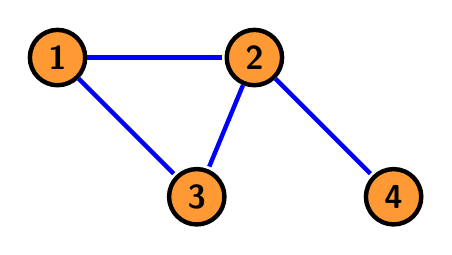
\begin{tikzpicture}[scale=0.1, 
	shorten >=1pt, 
	node distance=2.5cm, 
	ultra thick,
 	node_style/.style={
 	    circle,
 	    draw=black,
 	    fill=orange!80!,
 	    font=\sffamily\large\bfseries
 	    }, 
 	    minimum size=0.05cm, 
 		edge_style/.style={
 		draw=black, 
 		ultra thick, font=\Large
 		}
 	]
 	    % all the nodes
 		\node[node_style](1) {1};
 		\node[node_style, right of=1](2)  {2};
 		\node[node_style, below right of=1](3)  {3};
 		\node[node_style, right of=3](4)  {4};
 		
 		\draw[edge_style, draw=blue] (1) edge (2);
 		\draw[edge_style, draw=blue] (1) edge (3);
 		\draw[edge_style, draw=blue] (2) edge (3);
 		\draw[edge_style, draw=blue] (2) edge (4);
 		\end{tikzpicture}	
 		\caption{Undirected graph}
 		\label{undirected_net}
\end{figure}

\begin{figure}[htb]
    \centering
    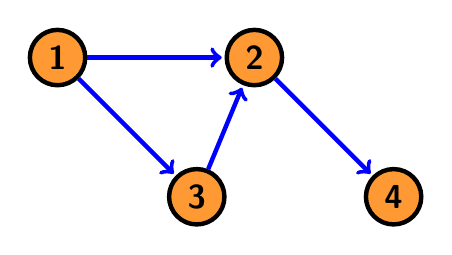
\begin{tikzpicture}[
    scale=0.1, 
    shorten >=1pt, 
    node distance=2.5cm, 
    ultra thick,			
    node_style/.style={
        circle,
        draw=black,
        fill=orange!80!,
        font=\sffamily\large\bfseries
        },
    minimum size=0.05cm,
 	edge_style/.style={
    	draw=black, 
 		ultra thick, 
 		font=\Large
 	}]
 			
 		\node[node_style](1) {1};
 		\node[node_style, right of=1](2)  {2};
 		\node[node_style, below right of=1](3)  {3};
 		\node[node_style, right of=3](4)  {4};
 		
 		\draw[edge_style, ->, draw=blue] (1) edge (2);
 		\draw[edge_style, ->, draw=blue] (1) edge (3);
 		\draw[edge_style, ->, draw=blue] (3) edge (2);
 		\draw[edge_style, ->, draw=blue] (2) edge (4);	
 	\end{tikzpicture}
    \caption{A directed graph}
    \label{fig:directed}
\end{figure}

\begin{figure}[htb]
    \centering
    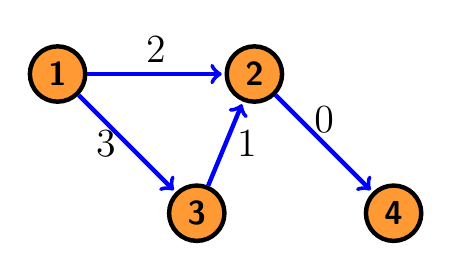
\begin{tikzpicture}[
    scale=0.1, 
    shorten >=1pt, 
    node distance=2.5cm, 
    ultra thick,			
    node_style/.style={
        circle,
        draw=black,
        fill=orange!80!,
        font=\sffamily\large\bfseries
        },
    minimum size=0.05cm,
 	edge_style/.style={
    	draw=black, 
 		ultra thick, 
 		font=\Large
 	}]
 			
 		\node[node_style](1) {1};
 		\node[node_style, right of=1](2)  {2};
 		\node[node_style, below right of=1](3)  {3};
 		\node[node_style, right of=3](4)  {4};
 		
 		\draw[edge_style, ->, draw=blue] (1) edge[above] node{2} (2);
 		\draw[edge_style, ->, draw=blue] (1) edge[left] node{3} (3);
 		\draw[edge_style, ->, draw=blue] (3) edge[right] node{1} (2);
 		\draw[edge_style, ->, draw=blue] (2) edge[above] node{0} (4);	
 	\end{tikzpicture}
    \caption{A weighted graph}
    \label{fig:weighted}
\end{figure}


\begin{figure}[htb]
    \centering
    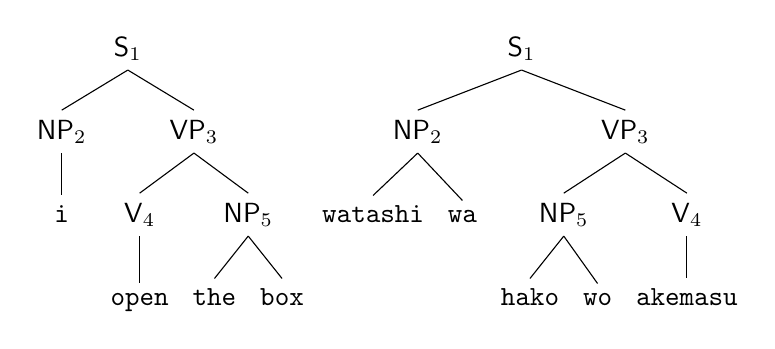
\begin{tikzpicture}
  \Tree 
  [.\textsf{S}$_1$ 
    [.\textsf{NP}$_2$ \texttt{i} ] [.\textsf{VP}$_3$ 
                    [.\textsf{V}$_4$ \texttt{open} ] [.\textsf{NP}$_5$                    \texttt{the} \texttt{box} ] ] ] ] ]

\begin{scope}[xshift=5cm]
  \Tree 
  [.\textsf{S}$_1$ 
    [.\textsf{NP}$_2$ \texttt{watashi} \texttt{wa} ] [.\textsf{VP}$_3$ 
                    [.\textsf{NP}$_5$ \texttt{hako} \texttt{wo} 
                    ] [.\textsf{V}$_4$                    \texttt{akemasu} ] ] ] ] ]
\end{scope}
\end{tikzpicture}
    \caption{Tree}
    \label{fig:tree}
\end{figure}


\end{document}